\documentclass{jsarticle}

%----------------------------------
% 文章の中に 画像を入れるための設定
%----------------------------------
\usepackage[dvipdfmx]{graphicx}

%----------------------------------
% 自分の作る文章の題
%----------------------------------
\title{上腕三頭筋の働きと鍛え方}

%---------------------------------- 
% 文書を作った日
%----------------------------------
\date{\today}

%----------------------------------
% 自分の名前を入れる
%----------------------------------
\author{山 根 千 佳}

%---------------------------------------------------
% 文書のスタイルを決める設定
%---------------------------------------------------
\usepackage[height=26cm,width=16cm]{geometry}

%-----------------------------------
% 以上で下準備は終わりです.
% ここから表示される文章を作成していきます.
%-----------------------------------
\begin{document}

%----------------------------------------
% 文章に上に、上記で記述したタイトル、
% 文書を作成した日にち, 著者の名前を書き込みます.
%
% (注)\maketitle をはずせば, タイトル, 日にち,著者名は文書に挿入されません.
%----------------------------------------

\maketitle

%--------------------------------------------
% 主な内容はここから
%--------------------------------------------

\section{目的}
本レポートは、腕の曲げ伸ばし運動における上腕二頭筋と上腕三頭筋の役割を推測することを目的とした。具体的には、腕の曲げ伸ばし運動における筋電位の変化と、腕の各関節の位置変化とを同時に計測することで、それらにどのような相関があるかを調べた。

\section{実験方法}
被験者は、膝をついた状態で座り、腕を床と水平に繰り返し曲げ伸ばしした。
計測は、腕の伸縮をゆっくり行った場合と、早く行った場合との2パターンについて行った。
本実験における被験者は1人であった。

\subsection{計測実験}
実験には、MotionCapture(ライブラリ社 MoveTR)と筋電計(ロジカルプロダクト社)を用いた。
MotionCaptureでは、被験者の運動の様子を真上からカメラで撮影し、肩、肘、手首の3点を追跡することで、各関節の位置座標の変化を計測した。このとき、$fps = 200$ とした。

また、筋電計は上腕二頭筋および上腕三頭筋に貼付し、各筋電データを取得した。このときのサンプリング周波数は1000とした。

\subsection{取得データの解析}
筋電データには、1〜40 Hzのバンドパスフィルタ(signal.buttord 関数)をかけた。また、バンドパスフィルタをかけることにより生じる時間のずれを、filtfit 関数により自動補正した。このデータをもとに、時刻$t$における筋肉の活動度$a(t)$を、
$$a(t) = \frac{1}{\Delta T} \int_{t-\frac{\Delta T}{2}}^{t+\frac{\Delta T}{2}} |E(t)|dt $$
として求めた。つまり、ある時刻$t$における筋肉の活動度を、その前後$\Delta T/2 = 5$ [ms]のデータ値を平均することで求めた。
これにより、生データにおける波形の不規則さが残らないように平滑化した。このとき、筋収縮の変化に追いつけるよう、$\Delta T$の値が大きくなりすぎないように注意した。

\clearpage
\section{結果}

\begin{figure}[h]
	\begin{center} %センタリングする
		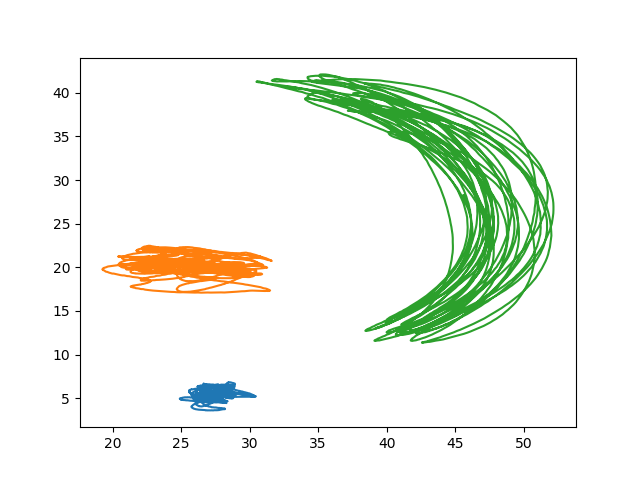
\includegraphics[width=10cm]{graph_image/slow.png}
		\caption{腕の3関節の軌道} %タイトルをつける
		\label{fig:kidou} %ラベルをつけ図の参照を可能にする
	\end{center}
\end{figure}
図\ref{kidou}はゆっくりと腕の曲げ伸ばし運動を行った場合の、各関節の位置変化を示す。
水色、オレンジ、黄緑はそれぞれ、肩、肘、手首の軌道を示している。
この図から、今回の実験では、手首における変化が3関節の中でもっと大きい。また、手首において、Y軸方向への位置変化がX軸方向に比べて大きいことがわかる。そこで、本レポートでは、筋電データと、Y軸方向への手首の動きの相関に注目した。

\begin{figure}[!h]
	\begin{center}
		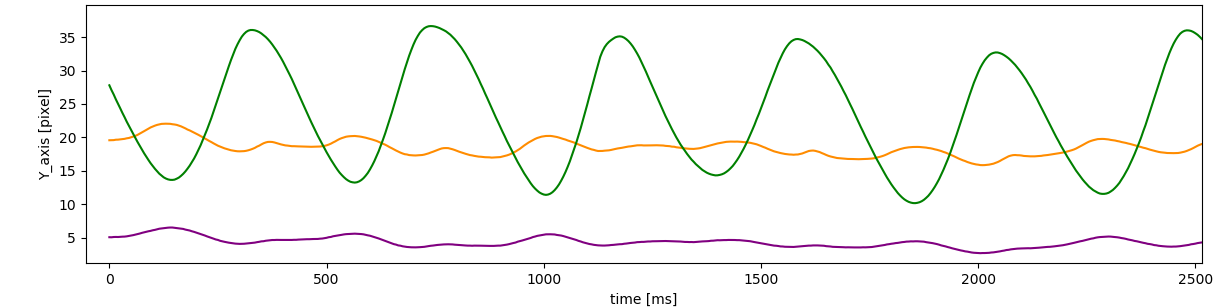
\includegraphics[width=17cm]{graph_image/fast_position.png}
		\caption{腕の曲げ伸ばし速度が速い時の各関節の位置変化}
		\label{fig:fast_position}
	\end{center}
\end{figure}


\begin{figure}[!h]
	\begin{center}
		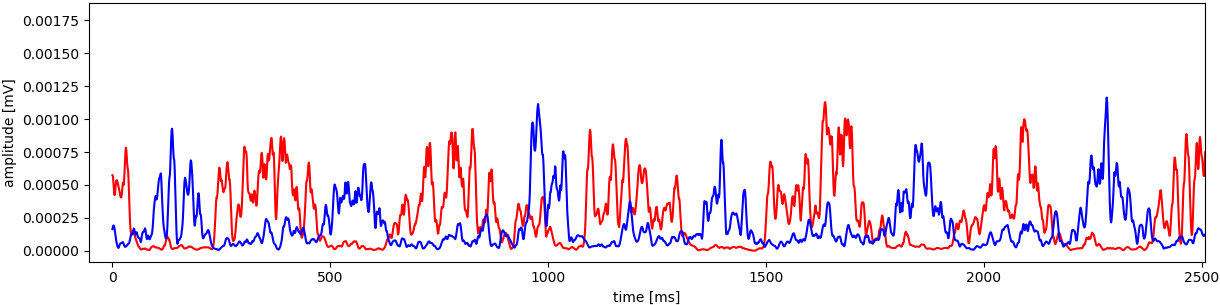
\includegraphics[width=17cm]{graph_image/fast_EMG.png}
		\caption{腕の曲げ伸ばし速度が速い時の筋電データ}
		\label{fig:fast_EMG}
	\end{center}
\end{figure}
\clearpage



\begin{figure}[!h]
	\begin{center}
		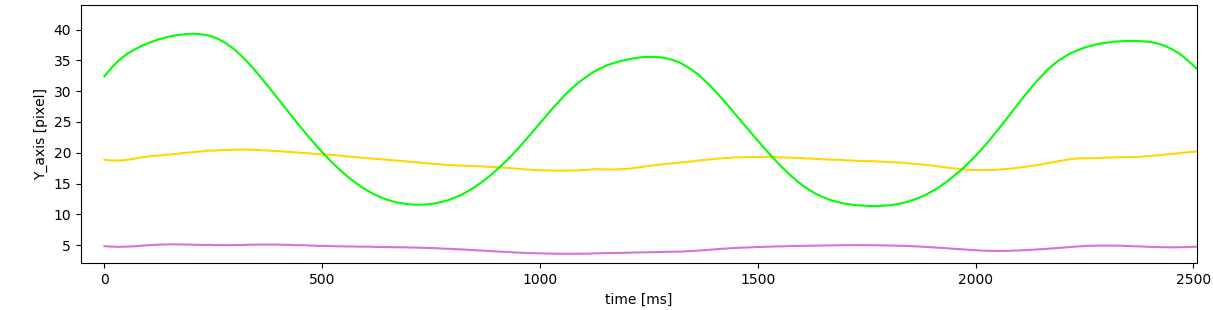
\includegraphics[width=17cm]{graph_image/slow_position.png}
		\caption{腕の曲げ伸ばし速度が遅い時の各関節の位置変化}
		\label{fig:slow_position}
	\end{center}
\end{figure}

\begin{figure}[!h]
	\begin{center}
		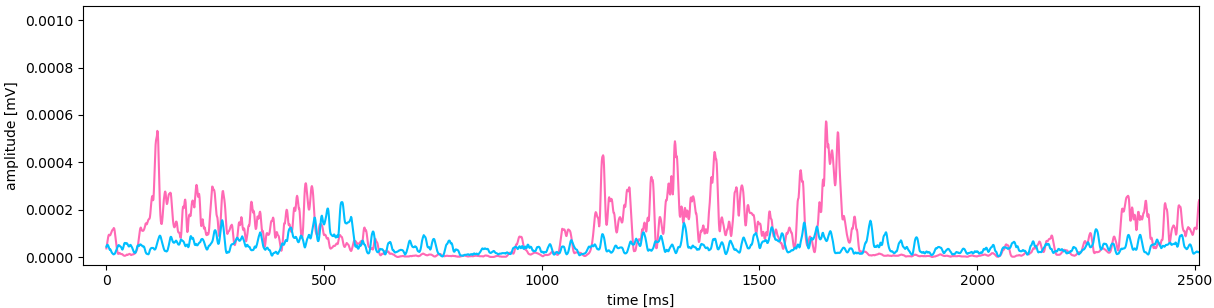
\includegraphics[width=17cm]{graph_image/slow_EMG.png}
		\caption{腕の曲げ伸ばし速度が遅い時の筋電データ}
		\label{fig:slow_EMG}
	\end{center}
\end{figure}


まず、腕の曲げ伸ばしが速い場合での計測結果について述べる。
図\ref{fig:fast_position}は、腕の曲げ伸ばし運動を速く行った場合の、各関節のY軸方向への時間変化である。紫、オレンジ、緑はそれぞれ肩、肘、手首の軌道を表す。
図\ref{fig:fast_EMG}は、赤が上腕二頭筋、青が上腕三頭筋の筋電データであり、縦軸は活動電位、横軸は時間である。
これら2つの図において、上腕二頭筋の筋電図は、Y軸方向の手首の動きと逆位相の形となっていた。つまり、腕が曲がる(手首がY軸下向きに移動する)ほど、より多くの筋繊維で活動電位が発生していることがわかる。また、速い腕の曲げ伸ばしでは、上腕二頭筋と上腕三頭筋のグラフがほぼ完全な逆位相になっていた。

次に、腕の曲げ伸ばしが遅い場合の計測結果について述べる。
図\ref{fig:slow_position}は、上段が腕の曲げ伸ばし運動を遅く行った場合のY軸方向の位置変化である。薄紫、黄色、黄緑はそれぞれ肩、肘、手首の位置変化を示す。
図\ref{fig:slow_EMG}は、ピンクが上腕二頭筋、水色が上腕三頭筋の筋電データである。
これらのグラフを比べると、遅い腕の曲げ伸ばしでは、上腕二頭筋と上腕三頭筋のグラフに位相のずれが生じているようにみえるが逆位相ではなかった。また、上腕二頭筋と上腕三頭筋のグラフの形が、腕の曲げ伸ばしが速いときのように似ておらず、上腕二頭筋の振幅が大きくなった後でも、それほど上腕三頭筋の振幅に変化が見られない部分も見られた。

上記以外にも、腕の曲げ伸ばしが速い場合と遅い場合で、グラフに違いが見られた。例えば、腕を速く動かした方が、遅く動かしたときよりも位置変化の周波数が高くなっている。また、上腕二頭筋の方が上腕三頭筋よりも大きな活動電位を発生させる傾向が見られ、腕の曲げ伸ばしが速い方が高い活動電位が見られた。

\section{考察}

本を読んでいると、上腕二頭筋は、腕を曲げる働きがあり、上腕三頭筋は腕を伸ばす働きがあるという情報があった\cite{reference}。しかし、腕の伸縮が遅い場合、上腕三頭筋には、上腕二頭筋に対応した大きな振幅を持つ部分が見られないこともあり、比較的平坦に近いグラフが出力された。このグラフでは、振幅は0に近かったが、完全に0となることはほとんどなかった。
私はこのことから、腕の伸縮が遅い場合のグラフでは、腕を伸ばすための活動電位に加えて、肩から腕までの部分を地面と水平に保持する筋力を発生させるための活動電位を見ているのではないかと考えた。つまり、上腕三頭筋には、肘を伸ばす役割の他に、肩から肘までの位置を固定・維持する役割があるのではないかと考えた。

また、腕を速く動かした場合の上腕三頭筋の筋電データが、Y軸方向における手首の位置変化から、腕を伸ばすときに上腕三頭筋での活動電位が大きくなることが確認できた。
これらのことから、上腕三頭筋を鍛えるためには、腕の曲げ伸ばし運動に加えて、肩から腕の位置固定を物理的に難しくするトレーニング(例えば、肩から腕までの部位に思いリングのようなものをかけた状態で腕を素早く曲げ伸ばしするなど)が有効なのではないかと考えられる。

\section{参考文献}
\begin{thebibliography}{9}
	\bibitem{reference} 「3D 踊る肉単」 河合良訓,原島広至 pp.xiv
\end{thebibliography}
%--------------------------------------------
% 文章これまで.
%--------------------------------------------
\end{document}
